\section{Methods Comparison and Related Work Review}

Swagat Kumar implemented a Deep Q Netword approach to this problem in 2020.
Their DQN result is shown below:

\begin{figure}[H] %h forces the figure to be inserted right here
    \centering
    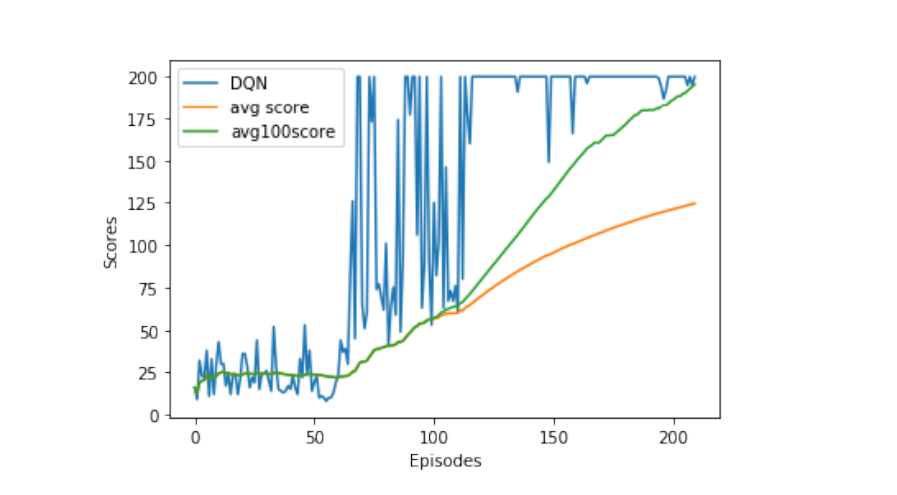
\includegraphics[width=0.75\linewidth]{kumar-2020-dqn.png}
    \caption{Performance of Kumar's DQN. Avg100score is the average of the last 100 episodes}
\end{figure}

It should be noted that Kumar used v0 of the CartPole environment, which has a much lower maximum reward threshold of 195. As such,
their model were able to solve the problem in only 200 episodes~\citep{kumar2020balancing}. Moreover, in the paper, Kumar also stated that
DQN is much faster compared to the usual Q-Learning approach, which solved the problem in 300 episodes.

We expect the same result would apply to our v1 environment, if we were to implement a Deep Q Network approach.

Another comparison is from~\citep{wang2013backward}. Here, Wang showed that SARSA performs slightly better than Q-Learning, taking less time to train, as shown
in this figure taken from the paper. From this figure, the Time factor will be taken into consideration.

\begin{figure}[H] %h forces the figure to be inserted right here
    \centering
    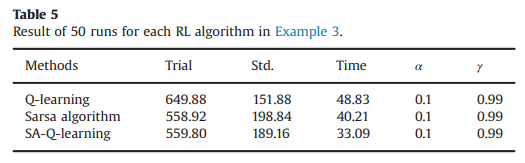
\includegraphics[width=0.75\linewidth]{wang-table.png}
    \caption{Performance of Wang's Algorithms}
\end{figure}

Compared to our implementation of SARSA and Q-Learning, where we have the average running time to go through 10000 episodes for Q Learning is 192.343 seconds, while SARSA takes 180.925 seconds to perform the same task.
So, our results matched that of Wang's, if running time is the only consideration. However, because of the difference in metrics, we considered Q Learning to be the better algorithm for our case.